\documentclass{beamer}

\usepackage[ruled]{algorithm2e}
\SetKw{KwRet}{return}
\SetKwRepeat{Repeat}{repeat}{until}
\usepackage{amsmath}

\usetheme{AnnArbor}
\usecolortheme{crane}
\usefonttheme[onlymath]{serif}

\title{Deep Learning - Foundations and Concepts}
\subtitle{Chapter 7. Gradient Descent}
\author{nonlineark@github}
\date{\today}

\begin{document}

\begin{frame}
    \titlepage
\end{frame}

\begin{frame}
    \frametitle{Outline}
    \tableofcontents
\end{frame}

\section{Error Surfaces}

\begin{frame}
    \frametitle{Gradient and stationary points}
    \begin{block}{Theorem}
        Let the function $f:\mathbb{R}^{n}\to\mathbb{R}$ be differentiable at $a\in\mathbb{R}^{n}$:
        \begin{enumerate}
            \item Near $a$ the function $f$ increases fastest in the direction of $\nabla{}f(a)\in\mathbb{R}^{n}$.
            \item The rate of increase in $f$ is measured by the length of $\nabla{}f(a)$.
            \item If $f$ has a local extremum at $a$ then $\nabla{}f(a)=0$.
        \end{enumerate}
    \end{block}
    \begin{block}{Definition}
        Let $f:\mathbb{R}^{n}\to\mathbb{R}$ be differentiable at $a\in\mathbb{R}^{n}$. Then $a$ is said to be a stationary point for $f$ if $Df(a)=0$, or, equivalently, $\nabla{}f(a)=0$.
    \end{block}
\end{frame}

\begin{frame}
    \frametitle{Gradient and stationary points}
    It's easy to see the correctness of the theorem. Since the rate of increase of $f$ at the point $a$ in an arbitray direction $v\in\mathbb{R}^{n}$ is given by the directional derivative at $v$, we have:
    \begin{equation*}
        |Df(a)v|=|v^{T}\nabla{}f(a)|\le||\nabla{}f(a)||||v||
    \end{equation*}
    where we have used the Cauchy-Schwarz inequality. The rate of increase is maximal if $v$ is a positive scalar multiple of $\nabla{}f(a)$. For the third claim, let's define $g_{j}$ as:
    \begin{equation*}
        g_{j}(t)=f(a_{1},\hdots,a_{j-1},t,a_{j+1},\hdots,a_{n})
    \end{equation*}
    then $g'_{j}(a_{j})=D_{j}f(a)$. Since $f$ has a local extremum at $a$, $g_{j}$ also has a local extremum at $a_{j}$. Thus $g'_{j}(a_{j})=0$ for $1\le{}j\le{}n$, and we have $\nabla{}f(a)=0$.
\end{frame}

\begin{frame}
    \frametitle{Gradient and stationary points}
    During training, we want to optimize the weights and biases $w\in\mathbb{R}^{W}$ by using a chosen error function $E(w)$. From the previous theorem we see that, its smallest value will occur at a point in weight space such that:
    \begin{equation*}
        \nabla{}E(w)=0
    \end{equation*}
    But:
    \begin{itemize}
        \item Global minimum vs. local minimum.
        \item For any point $w$ that is a local minimum, there will generally be other points in weight space that are equivalent minima (weight-space symmetries).
    \end{itemize}
\end{frame}

\begin{frame}
    \frametitle{Local quadratic approximation}
    \begin{block}{Threorem}
        Let $U$ be a convex open subset of $\mathbb{R}^{n}$ and let $a\in{}U$ be a stationary point for $f\in{}C^{2}(U)$. Then we have the following assertions:
        \begin{enumerate}
            \item If $Hf(a)$ is positive definite, then $f$ has a local strict minimum at $a$.
            \item If $Hf(a)$ is negative definite, then $f$ has a local strict maximum at $a$.
        \end{enumerate}
        where $Hf(a)$ is the Hessian of $f$ at $a$.
    \end{block}
\end{frame}

\begin{frame}
    \frametitle{Local quadratic approximation}
    We only prove the first claim. Using Taylor expansion, we see that:
    \begin{align*}
        f(a+h)&=f(a)+h^{T}\nabla{}f(a)+\frac{1}{2}h^{T}Hf(a)h+R_{2}(a,h) \\
        &=f(a)+\frac{1}{2}h^{T}Hf(a)h+R_{2}(a,h)
    \end{align*}
    where $\lim_{h\to{}0}\frac{R_{2}(a,h)}{||h||^{2}}=0$. Since $f\in{}C^{2}(U)$, $Hf(a)$ is a self-adjoint operator. Let $\lambda$ be its smallest eigenvalue. Because $Hf(a)$ is positive definite, $\lambda>0$. Notice that:
    \begin{itemize}
        \item $h^{T}Hf(a)h\ge\lambda||h||^{2}$.
        \item There is $\delta>0$, such that $\frac{|R_{2}(a,h)|}{||h||^{2}}<\frac{\lambda}{4}$ for $||h||<\delta$.
    \end{itemize}
    For $||h||<\delta$, we have:
    \begin{equation*}
        f(a+h)-f(a)=\frac{1}{2}h^{T}Hf(a)h+R_{2}(a,h)>\frac{\lambda}{2}||h||^{2}-\frac{\lambda}{4}||h||^{2}=\frac{\lambda}{4}||h||^{2}
    \end{equation*}
\end{frame}

\begin{frame}
    From the previous theorem, we see that: A necessary and sufficient condition for $w^{*}$ to be a local minimum of the error function $E(w)$ is that the gradient of $E(w)$ should vanish at $w^{*}$ and the Hessian matrix evaluated at $w^{*}$ should be positive definite.
    \begin{figure}
        \caption{Geometry of the error surface in the neighbourhood of a minimum $w^{*}$}
        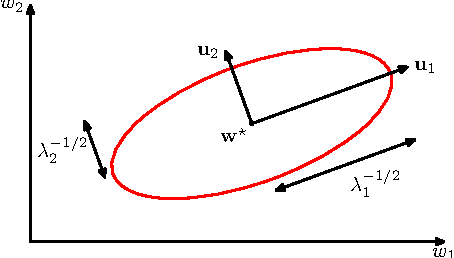
\includegraphics{Figure_2.pdf}
    \end{figure}
\end{frame}

\section{Gradient Descent Optimization}

\begin{frame}
    \frametitle{Use of gradient information}
    There is no way we can find an analytical solution to the equation $\nabla{}E(w)=0$, so we resort to iterative numerical procedures to minimize the error function:
    \begin{equation*}
        w^{(\tau)}=w^{(\tau-1)}+\Delta{}w^{(\tau-1)}
    \end{equation*}
\end{frame}

\begin{frame}
    \frametitle{Use of gradient information}
    Let's estimate the computational effort needed. The Taylor expansion of $E(w)$ around some point $\hat{w}$ in weight space is given by:
    \begin{equation*}
        E(w)\approx{}E(\hat{w})+(w-\hat{w})^{T}\nabla{}E(\hat{w})+\frac{1}{2}(w-\hat{w})^{T}HE(\hat{w})(w-\hat{w})
    \end{equation*}
    We see that in order to locate the minimum, we need at least $\mathcal{O}(W^{2})$ pieces of information, because:
    \begin{itemize}
        \item $\nabla{}E(\hat{w})$ contains $W$ independent parameters.
        \item $HE(\hat{w})$ contains $\frac{W(W+1)}{2}$ independent parameters.
    \end{itemize}
\end{frame}

\begin{frame}
    \frametitle{Use of gradient information}
    \begin{itemize}
        \item If we do not make use of gradient information, we would expect to have to perform $\mathcal{O}(W^{2})$ function evaluations, each of which would require $\mathcal{O}(W)$ steps. Thus the total cost would be $\mathcal{O}(W^{3})$.
        \item If we make use of the gradient information, each evaluation of $\nabla{}E$ brings $W$ pieces of information, so we would expect to find the minimum of the function in $\mathcal{O}(W)$ gradient evaluations. In the next chapter we shall see, by using error backpropagation, each such evaluation takes only $\mathcal{O}(W)$ steps. Thus the total cost would be $\mathcal{O}(W^{2})$.
    \end{itemize}
\end{frame}

\begin{frame}
    \frametitle{Batch gradient descent}
    The simplest approach to using gradient information is to take a small step in the direction of the negative gradient:
    \begin{equation*}
        w^{(\tau)}=w^{(\tau-1)}-\eta\nabla{}E(w^{(\tau-1)})
    \end{equation*}
    where the parameter $\eta>0$ is known as the learning rate. At each step:
    \begin{itemize}
        \item The weight vector is moved in the direction of the greatest rate of decrease of the error function ("gradient descent" in the name).
        \item The entire training set will be processed ("batch" in the name).
    \end{itemize}
\end{frame}

\begin{frame}
    \frametitle{Stochastic gradient descent}
    Note that error functions based on maximum likelihood for a set of independent observations comprise a sum of terms: $E(w)=\sum_{n=1}^{N}E_{n}(w)$. We can update the weight vector based on one data point at a time:
    \begin{equation*}
        w^{(\tau)}=w^{(\tau-1)}-\eta\nabla{}E_{n}(w^{(\tau-1)})
    \end{equation*}
    Advantages of stochastic gradient descent:
    \begin{itemize}
        \item It is much more efficient on very large data sets.
        \item It works when the data arises from a continuous stream of new data points (a.k.a., online algorithm).
        \item It handles redundancy in the data much more efficiently.
        \item The possibility of escaping from local minima.
    \end{itemize}
\end{frame}

\begin{frame}
    \frametitle{Stochastic gradient descent}
    \begin{algorithm}[H]
        \caption{Stochastic gradient descent}
        $n\gets{}1$\;
        \Repeat{convergence}{
            $w\gets{}w-\eta\nabla{}E_{n}(w)$\;
            $n\gets{}n+1(\mathrm{mod}N)$\;
        }
        \Return{$w$}\;
    \end{algorithm}
\end{frame}

\begin{frame}
    \frametitle{Mini-batches}
    \begin{algorithm}[H]
        \caption{Mini-batch stochastic gradient descent}
        $n\gets{}1$\;
        \Repeat{convergence}{
            $w\gets{}w-\eta\nabla{}E_{n:n+B-1}(w)$\;
            $n\gets{}n+B$\;
            \If{$n>N$}{
                shuffle data\;
                $n\gets{}1$\;
            }
        }
        \Return{$w$}\;
    \end{algorithm}
\end{frame}

\begin{frame}
    \frametitle{Parameter initialization}
    The initial setting for the parameters being learned can have a significant effect on:
    \begin{itemize}
        \item How long it takes to reach a solution.
        \item The generalization performance of the resulting trained network.
    \end{itemize}
    Although there is relatively little theory to guide the initialization strategy, one key consideration is symmetry breaking, by initializing parameters randomly from some distribution:
    \begin{itemize}
        \item Uniform distribution in the range $[-\epsilon,\epsilon]$.
        \item Zero-mean Gaussian of the form $\mathcal{N}(0,\epsilon^{2})$.
    \end{itemize}
\end{frame}

\begin{frame}
    \frametitle{Parameter initialization}
    The approach of He initialization for choosing the value of $\epsilon$. Consider a network in which layer $l$ evaluates the following transformations:
    \begin{align*}
        a^{(l)}_{i}&=\sum_{m=1}^{M}w_{im}z^{(l-1)}_{m} \\
        z^{(l)}_{i}&=\mathrm{ReLU}(a^{(l)}_{i})
    \end{align*}
    Suppose we initialize the weights using a Gaussian $\mathcal{N}(0,\epsilon^{2})$, and suppose that the pre-activations $a^{(l-1)}_{m}$ in layer $l-1$ have variance $\lambda^{2}$.
\end{frame}

\begin{frame}
    \frametitle{Parameter initialization}
    We see that:
    \begin{align*}
        E(a^{(l)}_{i})&=\sum_{m=1}^{M}E(w_{im})E(z^{(l-1)}_{m})=0 \\
        \mathrm{var}(a^{(l)}_{i})&=E((a^{(l)}_{i})^{2})-(E(a^{(l)}_{i}))^{2}=E((a^{(l)}_{i})^{2}) \\
        &=E(\sum_{1\le{}m,n\le{}M}w_{im}w_{in}z^{(l-1)}_{m}z^{(l-1)}_{n})=E(\sum_{m=1}^{M}w_{im}^{2}(z^{(l-1)}_{m})^{2}) \\
        &=\sum_{m=1}^{M}E(w_{im}^{2})E((z^{(l-1)}_{m})^{2})=\sum_{m=1}^{M}\epsilon^{2}\frac{1}{2}E((a^{(l-1)}_{m})^{2}) \\
        &=\sum_{m=1}^{M}\epsilon^{2}\frac{1}{2}\lambda^{2}=\frac{M}{2}\epsilon^{2}\lambda^{2}
    \end{align*}
\end{frame}

\begin{frame}
    \frametitle{Parameter initialization}
    If we require that the pre-activations at layer $l$ also have variance $\lambda^{2}$ then we arrive at the following choice for $\epsilon$ to initialize the weights that feed into a unit with $M$ inputs:
    \begin{equation*}
        \epsilon=\sqrt{\frac{2}{M}}
    \end{equation*}
    The bias parameters are typically set to small positive values to ensure that most pre-activations are initally active during learning.
\end{frame}

\section{Convergence}

\begin{frame}
    \frametitle{The rate of convergence}
    When applying gradient descent in practice, we need to choose a value for the learning parameter $\eta$:
    \begin{itemize}
        \item Increasing the value of $\eta$ may lead to oscillations, and if we increase $\eta$ too much, those oscillations will become divergent.
        \item So $\eta$ must be kept sufficiently small, gradient descent then takes many small steps to reach the minimum and is a very inefficient procedure.
    \end{itemize}
\end{frame}

\begin{frame}
    \frametitle{The rate of convergence}
    Consider the local quadratic approximation around a point $w^{*}$ that is a minimum of the error function:
    \begin{align*}
        E(w)&=E(w^{*})+\frac{1}{2}(w-w^{*})^{T}HE(w^{*})(w-w^{*}) \\
        \nabla{}E(w)&=HE(w^{*})(w-w^{*})
    \end{align*}
    And there is an orthogonal matrix $U$ that will diagonalize $HE(w^{*})$: $\Lambda=U^{T}HE(w^{*})U$. Under this new orthonormal basis where the transformation is given by $w-w^{*}=Uu$, we see that:
    \begin{align*}
        \Delta{}u&=U^{T}\Delta{}w=U^{T}(-\eta\nabla{}E(w))=-\eta{}U^{T}HE(w^{*})(w-w^{*}) \\
        &=-\eta{}U^{T}(U\Lambda{}U^{T})Uu=-\eta\Lambda{}u
    \end{align*}
\end{frame}

\begin{frame}
    \frametitle{The rate of convergence}
    For the $i$th coordinate, this is simply:
    \begin{align*}
        \Delta{}u_{i}&=-\eta\lambda_{i}u_{i} \\
        u_{i}^{\textrm{new}}&=(1-\eta\lambda_{i})u_{i}^{\textrm{old}} \\
        u_{i}^{(T)}&=(1-\eta\lambda_{i})^{T}u_{i}^{(0)}
    \end{align*}
    It follows that, provided $|1-\eta\lambda_{i}|<1$, the limit $T\to\infty$ leads to $u_{i}=0$, which means $w=w^{*}$, and so the weight vector has reached the minimum of the error. Further we see that:
    \begin{itemize}
        \item Convergence to the stationary point requires that all the $\lambda_{i}$ be positive.
        \item The value of $\eta$ has to be $\eta<\frac{2}{\lambda_{\textrm{max}}}$ where $\lambda_{\textrm{max}}$ is the largest of the eigenvalues.
        \item The rate of convergence is dominated by the smallest eigenvalue.
    \end{itemize}
\end{frame}

\begin{frame}
    \frametitle{Momentum}
    One simple technique for dealing with the problem of widely differing eigenvalues is to add a momentum term to the gradient descent formula:
    \begin{equation*}
        \Delta{}w^{(\tau-1)}=-\eta\nabla{}E(w^{(\tau-1)})+\mu\Delta{}w^{(\tau-2)}
    \end{equation*}
    To understand the effect of the momentum term, let's consider two cases:
    \begin{itemize}
        \item If the error surface has relatively low curvature ($\nabla{}E(w)$ is almost constant): $\Delta{}w=-\eta\nabla{}E(1+\mu+\mu^{2}+\cdots)=-\frac{\eta}{1-\mu}\nabla{}E$. We see the effective learning rate is increased from $\eta$ to $\frac{\eta}{1-\mu}$.
        \item If the error surface has high curvature in which the gradient descent is oscillatory, successive contributions from the momentum term will tend to cancel and the effective learning rate will be close to $\eta$.
    \end{itemize}
\end{frame}

\begin{frame}
    \frametitle{Momentum}
    \begin{figure}
        \caption{The effect of the momentum term}
        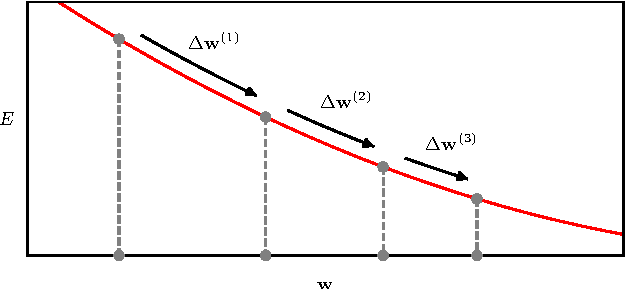
\includegraphics[height=0.4\textheight]{Figure_4.pdf}
        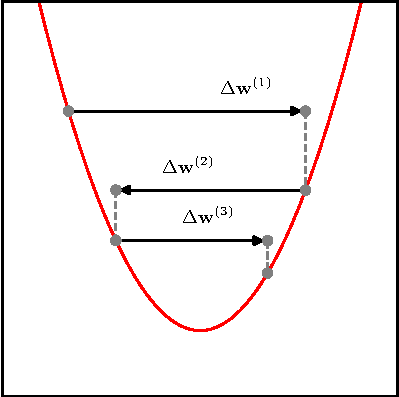
\includegraphics[height=0.4\textheight]{Figure_5.pdf}
    \end{figure}
\end{frame}

\begin{frame}
    \frametitle{Momentum}
    \begin{algorithm}[H]
        \caption{Stochastic gradient descent with momentum}
        $n\gets{}1$\;
        $\Delta{}w\gets{}0$\;
        \Repeat{convergence}{
            $\Delta{}w\gets-\eta\nabla{}E_{n:n+B-1}(w)+\mu\Delta{}w$\;
            $w\gets{}w+\Delta{}w$\;
            $n\gets{}n+B$\;
            \If{$n>N$}{
                suffle data\;
                $n\gets{}1$\;
            }
        }
        \Return{$w$}\;
    \end{algorithm}
\end{frame}

\begin{frame}
    \frametitle{Learning rate schedule}
    To specify a value for the learning rate parameter $\eta$, in practice, the best results are obtained by using a larger value for $\eta$ at the start of training and then reducing the learning rate over time:
    \begin{equation*}
        w^{(\tau)}=w^{(\tau-1)}-\eta^{(\tau-1)}\nabla{}E_{n}(w^{(\tau-1)})
    \end{equation*}
    Here are some examples of learning rate schedules:
    \begin{align*}
        \eta^{(\tau)}&=(1-\frac{\tau}{K})\eta^{(0)}+\frac{\tau}{K}\eta^{(K)} \\
        \eta^{(\tau)}&=\eta^{(0)}(1+\frac{\tau}{s})^{c} \\
        \eta^{(\tau)}&=\eta^{(0)}c^{\frac{\tau}{s}}
    \end{align*}
\end{frame}

\begin{frame}
    \frametitle{RMSProp and Adam}
    The optimal learning rate depends on the local curvature of the error surface. There are several algorithms that use different learning rates for each parameter in the network.
    \bigbreak
    AdaGrad (adaptive gradient):
    \begin{align*}
        r^{(\tau)}_{i}&=r^{(\tau-1)}_{i}+(\frac{\partial{}E(w)}{\partial{}w^{(\tau-1)}_{i}})^{2} \\
        w^{(\tau)}_{i}&=w^{(\tau-1)}_{i}-\frac{\eta}{\sqrt{r^{(\tau)}_{i}}+\delta}\frac{\partial{}E(w)}{\partial{}w^{(\tau-1)}_{i}}
    \end{align*}
\end{frame}

\begin{frame}
    \frametitle{RMSProp and Adam}
    RMSProp (root mean square propagation):
    \begin{align*}
        r^{(\tau)}_{i}&=\beta{}r^{(\tau-1)}_{i}+(1-\beta)(\frac{\partial{}E(w)}{\partial{}w^{(\tau-1)}_{i}})^{2} \\
        w^{(\tau)}_{i}&=w^{(\tau-1)}_{i}-\frac{\eta}{\sqrt{r^{(\tau)}_{i}}+\delta}\frac{\partial{}E(w)}{\partial{}w^{(\tau-1)}_{i}}
    \end{align*}
    where $0<\beta<1$ and a typical value is $\beta=0.9$.
\end{frame}

\begin{frame}
    \frametitle{RMSProp and Adam}
    Adam (adaptive moments):
    \begin{align*}
        s^{(\tau)}_{i}&=\beta_{1}s^{(\tau-1)}_{i}+(1-\beta_{1})\frac{\partial{}E(w)}{\partial{}w^{(\tau-1)}_{i}} \\
        r^{(\tau)}_{i}&=\beta_{2}r^{(\tau-1)}_{i}+(1-\beta_{2})(\frac{\partial{}E(w)}{\partial{}w^{(\tau-1)}_{i}})^{2} \\
        \hat{s}^{(\tau)}_{i}&=\frac{s^{(\tau)}_{i}}{1-\beta_{1}^{\tau}} \\
        \hat{r}^{(\tau)}_{i}&=\frac{r^{(\tau)}_{i}}{1-\beta_{2}^{\tau}} \\
        w^{(\tau)}_{i}&=w^{(\tau-1)}_{i}-\frac{\eta}{\sqrt{\hat{r}^{(\tau)}_{i}}+\delta}\hat{s}^{(\tau)}_{i}
    \end{align*}
    where $0<\beta_{1},\beta_{2}<1$ and typical values for them are $\beta_{1}=0.9$ and $\beta_{2}=0.99$.
\end{frame}

\begin{frame}
    \frametitle{RMSProp and Adam}
    \begin{algorithm}[H]
        \caption{Adam optimization}
        $n\gets{}1,\tau\gets{}1,s\gets{}0,r\gets{}0$\;
        \Repeat{convergence}{
            $g=\nabla{}E_{n:n+B-1}(w)$\;
            $s\gets\beta_{1}s+(1-\beta_{1})g,r\gets\beta_{2}r+(1-\beta_{2})g*g$\;
            $\hat{s}\gets\frac{s}{1-\beta_{1}^{\tau}},\hat{r}\gets\frac{r}{1-\beta_{2}^{\tau}}$\;
            $w\gets{}w-\frac{\eta}{\sqrt{\hat{r}}+\delta}\hat{s}$\;
            $n\gets{}n+B,\tau\gets\tau+1$\;
            \If{$n>N$}{
                shuffle data\;
                $n\gets{}1$\;
            }
        }
        \Return{$w$}\;
    \end{algorithm}
\end{frame}

\end{document}